\documentclass{edm_template}

\usepackage{url}

\begin{document}

\title{Choosing Sample Size for Knowledge Tracing Models
\titlenote{This is a submitted draft to the BKT20y Workshop (2014). This is not a peer-reviewed work.}}
%\subtitle{[Extended Abstract]
%\titlenote{A full version of this paper is available as
%\textit{Author's Guide to Preparing ACM SIG Proceedings Using
%\LaTeX$2_\epsilon$\ and BibTeX} at
%\texttt{www.acm.org/eaddress.htm}}}

\numberofauthors{1}
\author{
\alignauthor
Derrick Coetzee\\
       \affaddr{University of California, Berkeley}\\
       \email{dcoetzee@berkeley.edu}
}

\maketitle
\begin{abstract}
An important question in the practical application of Bayesian knowledge
tracing models is determining how much data is needed to infer
parameters accurately. If training data is inadequate, even a perfect
inference algorithm will produce parameters with poor predictive
power. In this work, we describe an empirical study using synthetic
data that provides estimates of the accuracy of inferred parameters
based on factors such as the number of students used to train the model,
and the values of the underlying generating parameters. We find that
the standard deviation of the error is roughly proportional to $1/\sqrt{n}$ where
$n$ is the sample size, and that model parameters near 0 and 1 are easier
to learn accurately.
\end{abstract}

%% A category with the (minimum) three required fields
\category{H.2.8}{Database Applications}{Data Mining}
%\category{H.4}{Information Systems Applications}{Miscellaneous}
%%A category including the fourth, optional field follows...
%\category{D.2.8}{Software Engineering}{Metrics}[complexity measures, performance measures]
%
\terms{Measurement,Theory.}

\keywords{Educational data mining,knowledge tracing,sample size}

% p3. Figure 3 - In this figure the Prior and Guess follow each other almost exactly. It is worth reflecting on this given Van de Sande’s analytic formulation of BKT as a 3 parameter model with Prior and Guess combined into a single parameter. % dcc - I don't think this is meaningful, their error varies at other parameter settings

\section{Introduction}
Simple Bayesian knowledge tracing models a student's observed responses to a sequence of items
as a Markov process, with their knowledge state as a hidden underlying variable. If values
are given for the four standard parameters, learning rate, prior, guess, and slip, the
likelihood of a particular set of response sequences can be computed. Using standard search
procedures like expectation maximization (EM), the parameter set giving the highest likelihood
for a given set of sequences can be determined, provided that the procedure converges to the global
maximum.

However, even if the procedure identifies the global maximum correctly and precisely, the resulting
parameters may not reflect the actual parameters that generated the data; this is a \emph{sampling error}
effect. It's clearest with very small samples, such as samples of size 1, but exists with larger samples as well. Empirical studies with synthetic data generated from known parameters show that the inferred parameters for a given data set can differ substantially from the generating parameters, and this same issue would arise in real settings. An understanding of the magnitude of sampling error in a particular scenario
can help to explain why the resulting model does or does not make effective predictions. Moreover, by providing
a means to describe the distribution of possible generating parameter values, the uncertainty of calculations based on those parameters such as predictions can also be determined.

\section{Related work}
For simple problems, such as identifying the mean value of a parameter in a population, or the proportion of the population falling into a subgroup, there are simple and well-understood statistical approaches for determining sample size based on statistical power. Such analytic approaches are not immediately applicable to the problem of minimizing the HMM error function because of its complexity and high dimensionality.

Falakmasir et al~\cite{falakmasir2013spectral} have noted that training time increases linearly with the size of the training set. Choosing an appropriate sample size for a certain desired level of accuracy can thus help to reduce training time, which is important both for research and in some real-time interactive tutor applications.

Nooraei et al~\cite{conf/edm/NooraeiPHB11} found that using only the 15 most recent data points from each student to train a knowledge tracing model yielded root mean-square error during prediction comparable to using the student's full history. For one data set, the most 5 recent items sufficed. Our study conversely does not vary the number of items per student, but instead varies the number of students and the four parameters generating the data. By allowing sample size to be reduced to meet a desired accuracy, our work offers an orthogonal method of further reducing training time.

De Sande~\cite{vandesande2013} has suggested that as samples become larger, models with small parameter sets  may no longer be rich enough to capture the sample's complexity. Thus our exclusive reliance on a simple four-parameter BKT model even for very large samples is a limitation of our approach.

\section{Methodology}

In our experiments we relied on a simple standard Bayesian knowledge tracing model with four parameters: learning rate, prior, guess and slip. There is only one value for each parameter, and no specialization by student or problem. Each synthetic student responded to five items; we do not vary this parameter in this study, since Nooraei et al~\cite{conf/edm/NooraeiPHB11} report that increasing this parameter has diminishing returns, but future work may investigate it.

We generate separate datasets for each of our experiments. In each case, we enumerate a sequence of models (each specified by values for learn, prior, guess, slip, sample size), and for each of those models, we generate a large number of random samples consistent with that model. For example, for a particular model, we may generate 1000 samples each containing 1000 students.

\begin{figure}
\centering
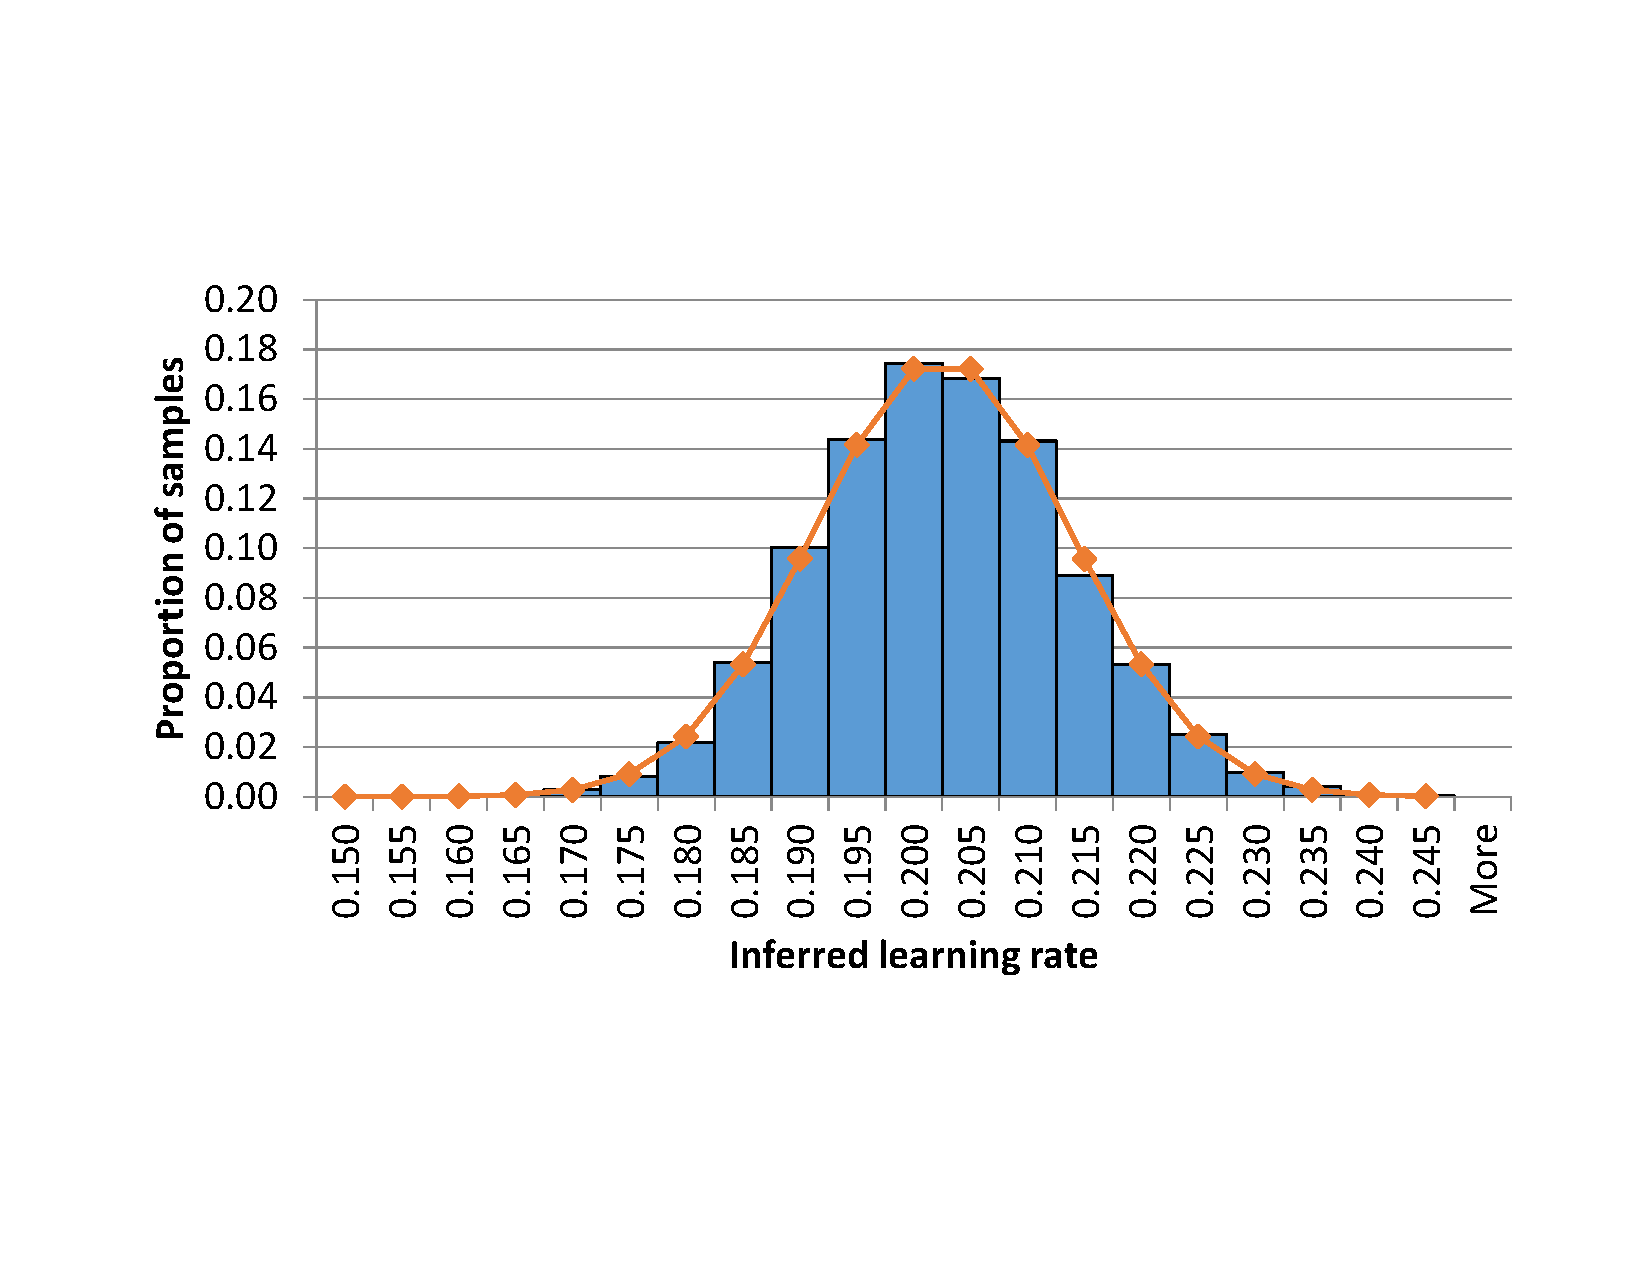
\includegraphics[width=0.5\textwidth]{data/normal.pdf}
\caption{Given the fixed model learn=0.2, prior=0.4, guess=0.14, slip=0.05, we generated 10000 samples with 1000 students each, and for each, inferred all four parameters using EM. The distribution of the inferred learning rate parameter over the samples is above. The mean differs by $3 \times 10^{-6}$ from the true generating parameter 0.2. The standard deviation is 0.01121, and the orange line shows the expected height of each bar if the proportions precisely followed a normal distribution. Scipy's normaltest~\cite{normaltest} rejects that the distribution is perfectly normal ($p < 0.0002$), and a small amount of negative (left) skew is visible; the median is 0.00016 smaller than the mean. But the distribution is close enough to normal for our purposes.}
\label{fig:normal}
\end{figure}

We then run EM on each sample to find the parameter set giving the maximum likelihood value. All parameters are permitted to vary during the search. EM is run starting at the generating parameters and run until fully converged (within $10^{-12}$ or until 100 iterations are complete). Starting at the generating parameters is not feasible in a realistic setting, but here it allows EM to run quickly and consistently reach the global minimum. As shown in Figure~\ref{fig:normal}, the parameter values inferred from these samples approximate a normal distribution with a mean equal to the generating parameter.

Finally, we take all samples generated from a single model and, for each parameter, record the mean and standard deviation of the inferred values for that parameter. We chose the number of samples generated for each model large enough so that these statistics remain stable under repeated runs. Mean values for each parameter were consistently near the generating parameter, typically within at most 0.1 standard deviations. Standard deviation provides an estimate of variation in the inferred parameter values, and is plotted. Different models yield different standard deviation values.

Because of the very large number of large samples involved in this approach, we use the \emph{fastHMM} C++ BKT library designed by Pardos and Johnson~\cite{pardosjohnson} to quickly generate datasets and perform EM, invoked from a Matlab script.

\subsection{Varying one parameter}
\label{variance1method}

In our first experiment, we start with typical, plausible values for all four parameters: learn=0.2, prior=0.4, guess=0.14, slip=0.05. These values are consistent with prior work that found large guess and slip values (> 0.5) to be implausible in most scenarios~\cite{ritter}, and in our 5-problem scenario, the chance of learning the material by the end is about 67\%, which is reasonable.

Then, for each of the four parameters, we hold the other parameters at their single plausible value, and vary the remaining parameter from 0 to 1 in steps of 0.01. This results in 404 total parameter sets.

For each parameter set, we generate 1000 random samples of 1000 students each. In this experiment, the number of students is fixed at 1000, which is large enough to consistently produce a standard deviation not exceeding 0.03 --- this avoids the boundary effects near 0 and 1 that would occur for very small samples.

In this experiment, we focus on the variance of our estimates of the parameter that is being varied, and don't consider variance of the other (fixed) parameters. 

\subsection{Interactions between parameters}
\label{variance2method}

In this experiment, similiar to the first, we hold three parameters fixed (learn=0.2, prior=0.4, guess=0.14), and vary slip between 0 and 1 in steps of 0.01. This gives 101 parameter sets. For each, we generate 1000 random samples of 1000 students each. However, in this experiment we examine variance of our estimates of all four parameters, rather than just the one being varied (slip). This experiment helps to demonstrate to what extent varying one parameter can affect the difficulty of accurately inferring other parameters.

\subsection{Varying sample size}
\label{variance3method}

In our third experiment, we fix the value of all four parameters, but vary the sample size in powers of two from 2 to 2097152. For sample sizes below 10000, we generate 1000 samples of that size, while for those above we generate 100 samples. The parameter values are heuristically chosen based on the prior experiments above to generate large error values (but not necessarily the worst possible error). We examine how variation of our estimates of all four parameters varies with sample size, and identify any trends.

\subsection{Interaction between sample size and parameters}
\label{variance4method}

In our final experiment, we vary both the learning rate (from 0 to 1 in steps of 0.01) and the sample size (between the values 1000, 10000, 100000) at the same time. This enables us to examine whether there is any interaction between parameters and sample size. For 1000 and 10000 students we use 1000 samples, while for 100000 students we use 100 samples, to reduce runtime.

\section{Results}

\subsection{Varying one parameter}
\label{variance1}

\begin{figure}
\centering
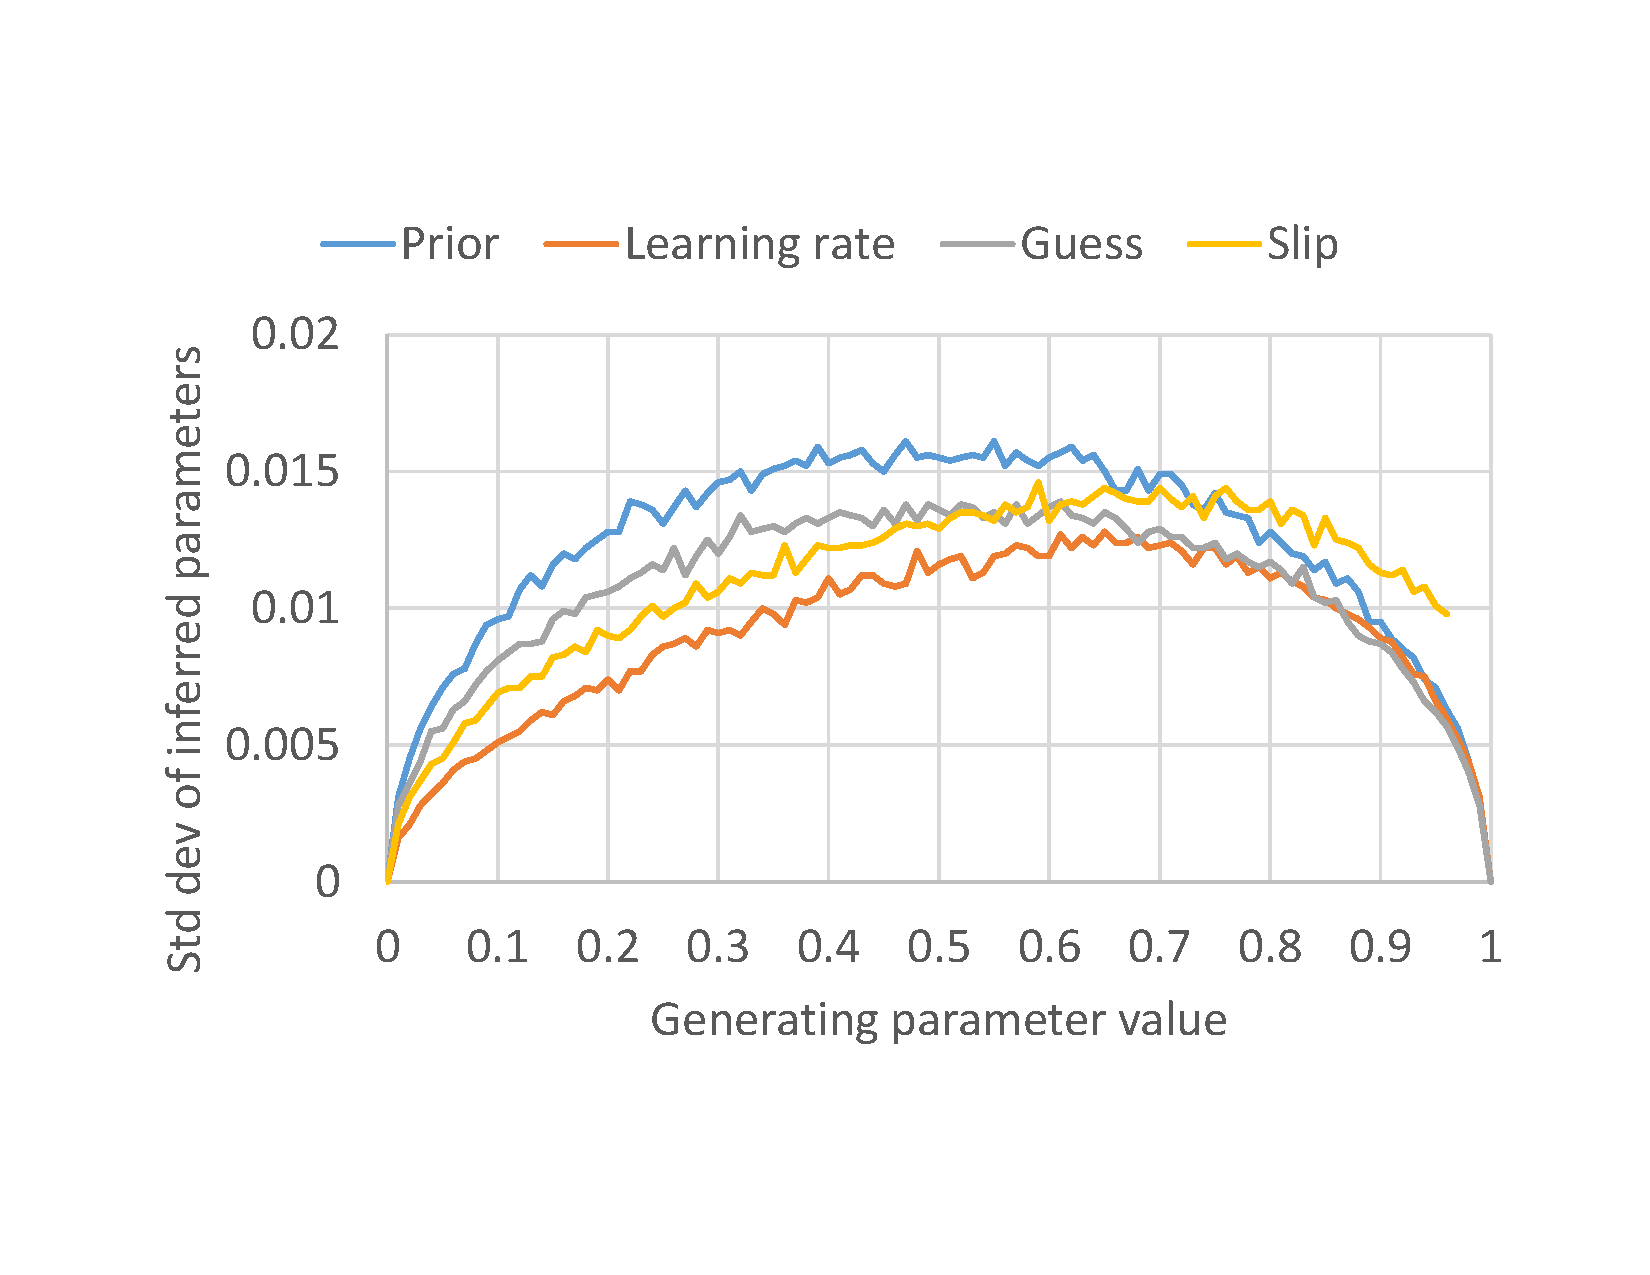
\includegraphics[width=0.5\textwidth]{data/variance1.pdf}
\caption{Variation of inferred parameters, based on underlying generating parameter. For each curve, all parameters other than one being examined are fixed at plausible values. Values near 0 and 1 are the easiest to infer accurately, and each parameter exhibits a unique pattern.}
\label{fig:variance1}
\end{figure}

As described in section~\ref{variance1method}, in this experiment we vary each parameter between 0 and 1 while holding the other parameters fixed, and examined how the variation in our inference of that parameter changed with its value. As shown in Figure~\ref{fig:variance1}, parameters with values near 0 or 1 are easier to accurately estimate, while those with values in the 0.4 to 0.8 range are more difficult to infer. Each parameter exhibits a unique pattern, with prior behaving worst for small values, guess behaving worst for values in the middle, and learning rate performing worst for the largest values. Slip is unique in having two peaks in its curve near 0.5 and 0.8.

\subsection{Interactions between parameters}
\label{variance2}

\begin{figure}
\centering
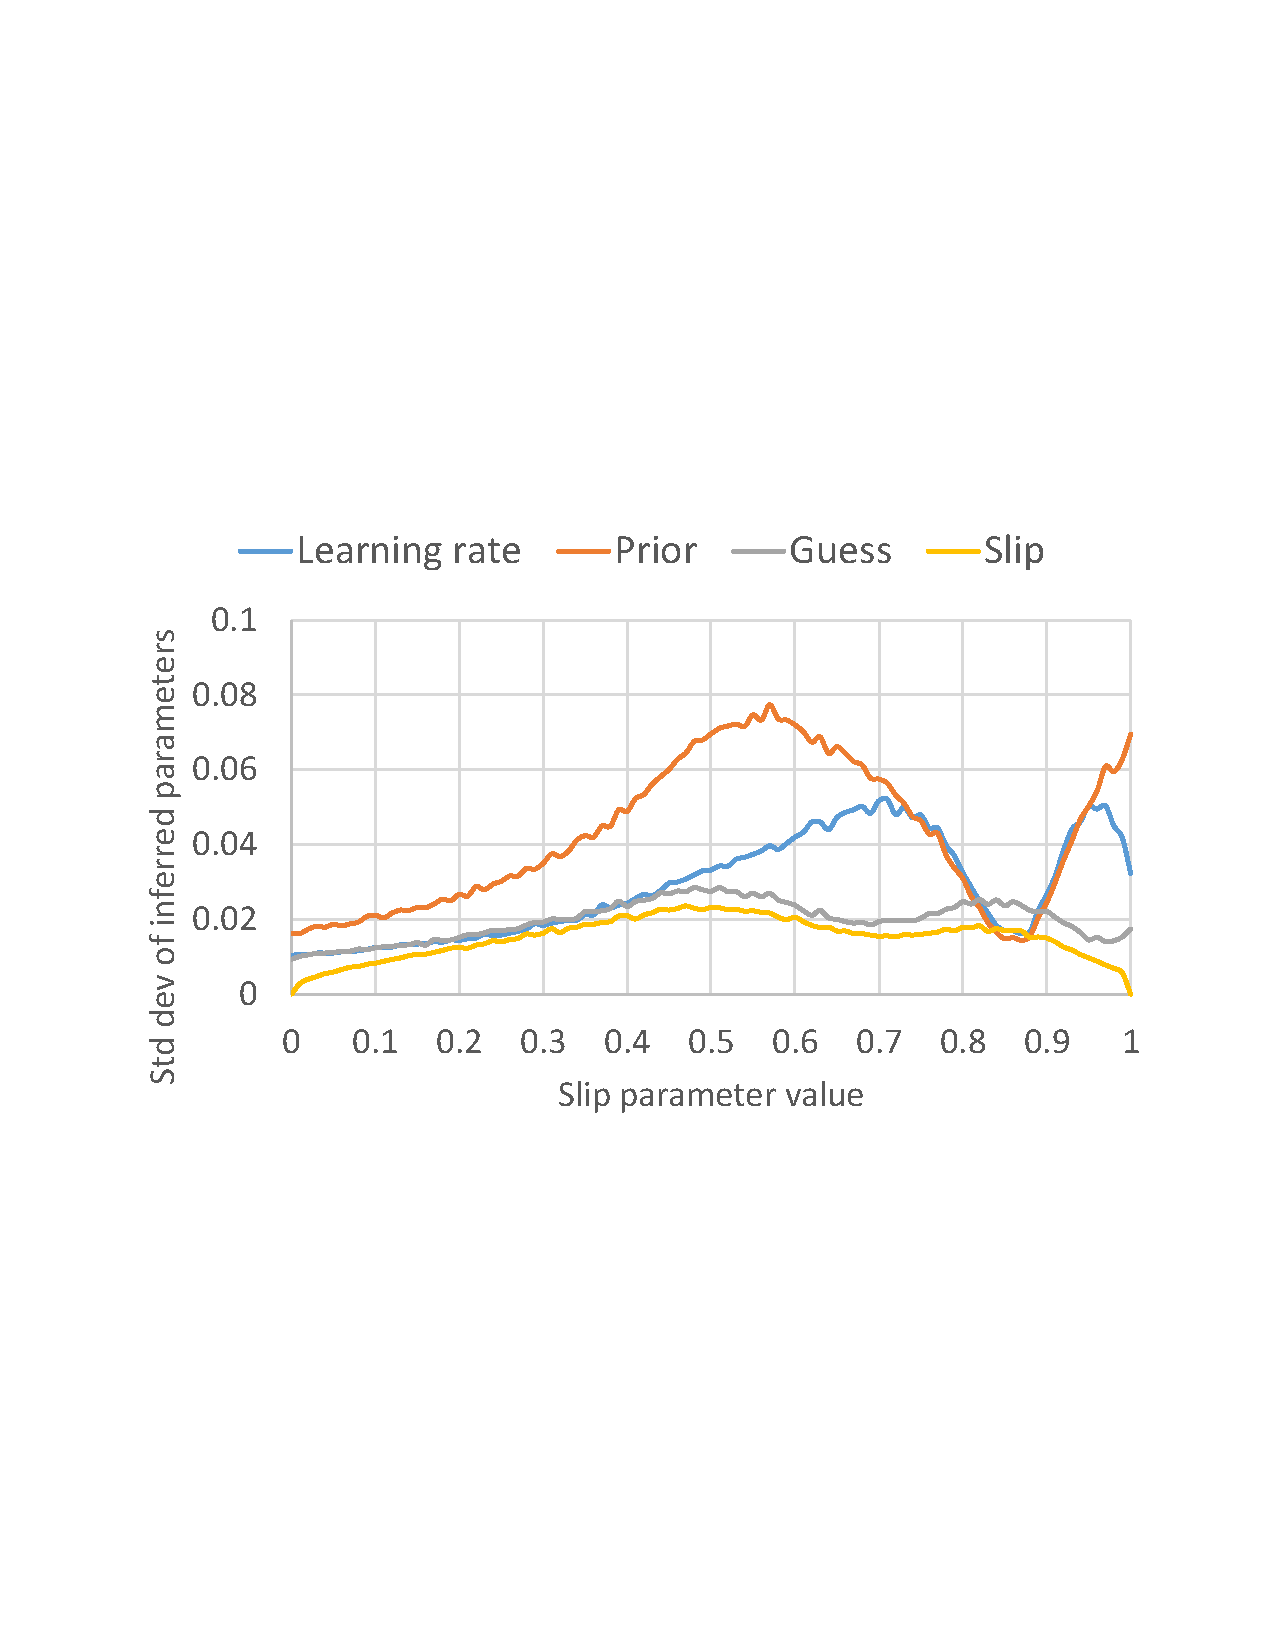
\includegraphics[width=0.5\textwidth]{data/variance2.pdf}
\caption{As the slip parameter is varied and the other parameters are held fixed (learn=0.2, prior=0.4, guess=0.14), the error in our inference of all other parameters varies in a strong and complex fashion, indicating interactions in the inference of different parameters.}
\label{fig:variance2}
\end{figure}

As described in section~\ref{variance2method}, in this experiment we vary slip between 0 and 1 while keeping the other parameters fixed, and examine how the variation of all four inferred parameters varies, as shown in Figure~\ref{fig:variance2}. All variance values exhibit a strong, complex dependence on the slip parameter---in particular there is a dramatic and unexpected drop from large variance to small variance around slip=0.85. We conclude that the variance of an inferred parameter depends not only on the value of that parameter, but also the values of other parameters.

\subsection{Varying sample size}

We fix the parameters at the values empirically determined in section~\ref{variance1} to give maximum variance (roughly based on the maximums of the curves, with prior and guess at 0.5, and learning rate and slip at 0.67). Because section~\ref{variance2} suggests that there are interactions between parameters, this may not give the worst-case variance possible of all combinations, but it is a reasonable starting point for realistic values.

\begin{figure}
\centering
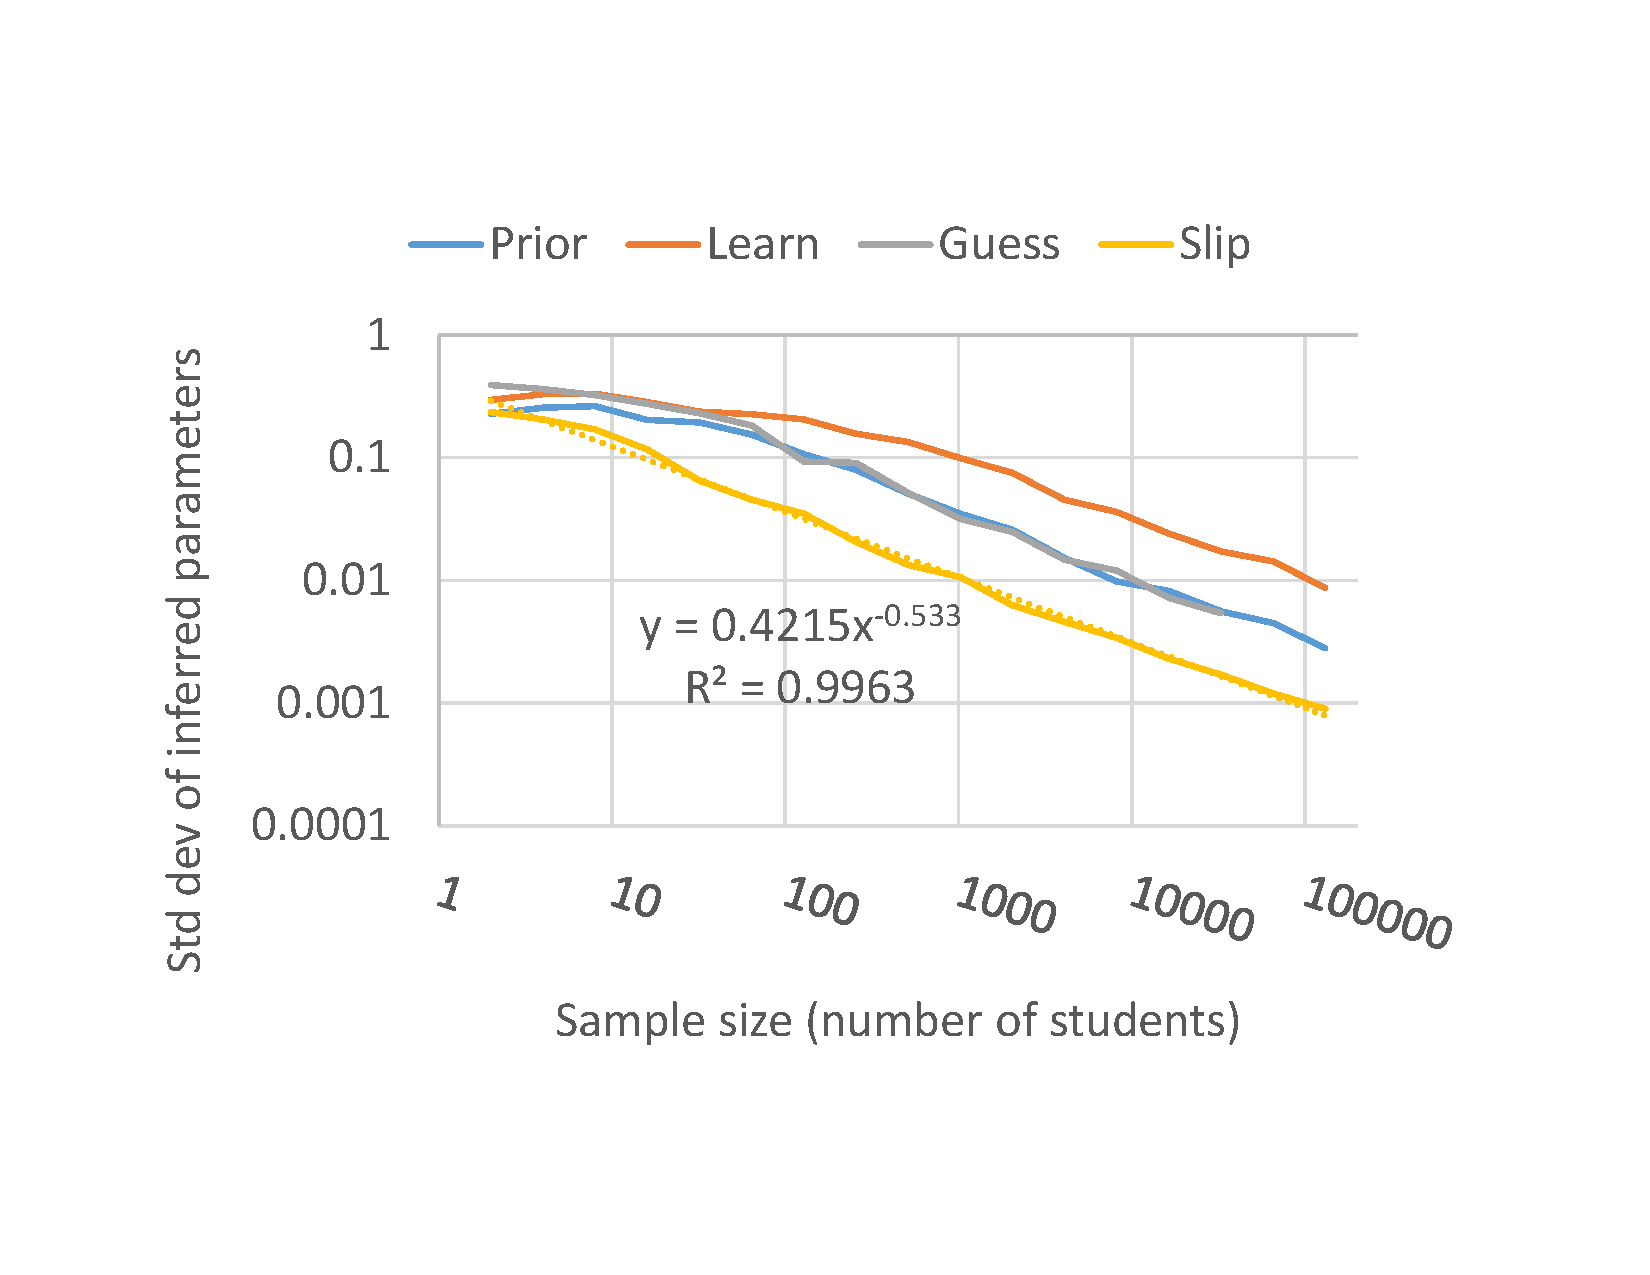
\includegraphics[width=0.5\textwidth]{data/variance3.pdf}
\caption{Accuracy of inferred parameters, based on sample size (training set size), with fixed parameters (prior=guess=0.5, learning=slip=0.67). This is a log-log plot, and (once the $y=0.1$ level is reached) the lines each remain straight and have slope of roughly -0.5. This suggests that the standard deviation of the error is roughly proportional to $1/\sqrt{n}$, where $n$ is the sample size.}
\label{fig:variance3}
\end{figure}

As described in section~\ref{variance3method}, sample size is varied in powers of two from 2 to 2097152. Figure~\ref{fig:variance3} shows the result, suggesting that (except for very small samples) the standard deviation of the error is roughly proportional to $n^{-0.5}$, or $1/\sqrt{n}$, where $n$ is the sample size. For these particular parameter values, slip is consistently inferred most accurately, learning rate is inferred least accurately, and guess and prior are between the two and are similar.

\subsection{Interaction between sample size and parameters}

In our final experiment, as described in section~\ref{variance4method}, we vary both the learning rate and the sample size at the same time. The standard deviation curves for the three sample sizes are then plotted on the same plot, each divided by the $1/\sqrt{n}$ factor, where $n$ is the sample size, as shown in Figure~\ref{fig:variance4}. The curves are nearly identical, and we find no evidence of interaction between parameters and sample size, but we can't rule out interaction for other combinations of parameter values. This also offers additional evidence for the $1/\sqrt{n}$ trend from the previous section.

\begin{figure}
\centering
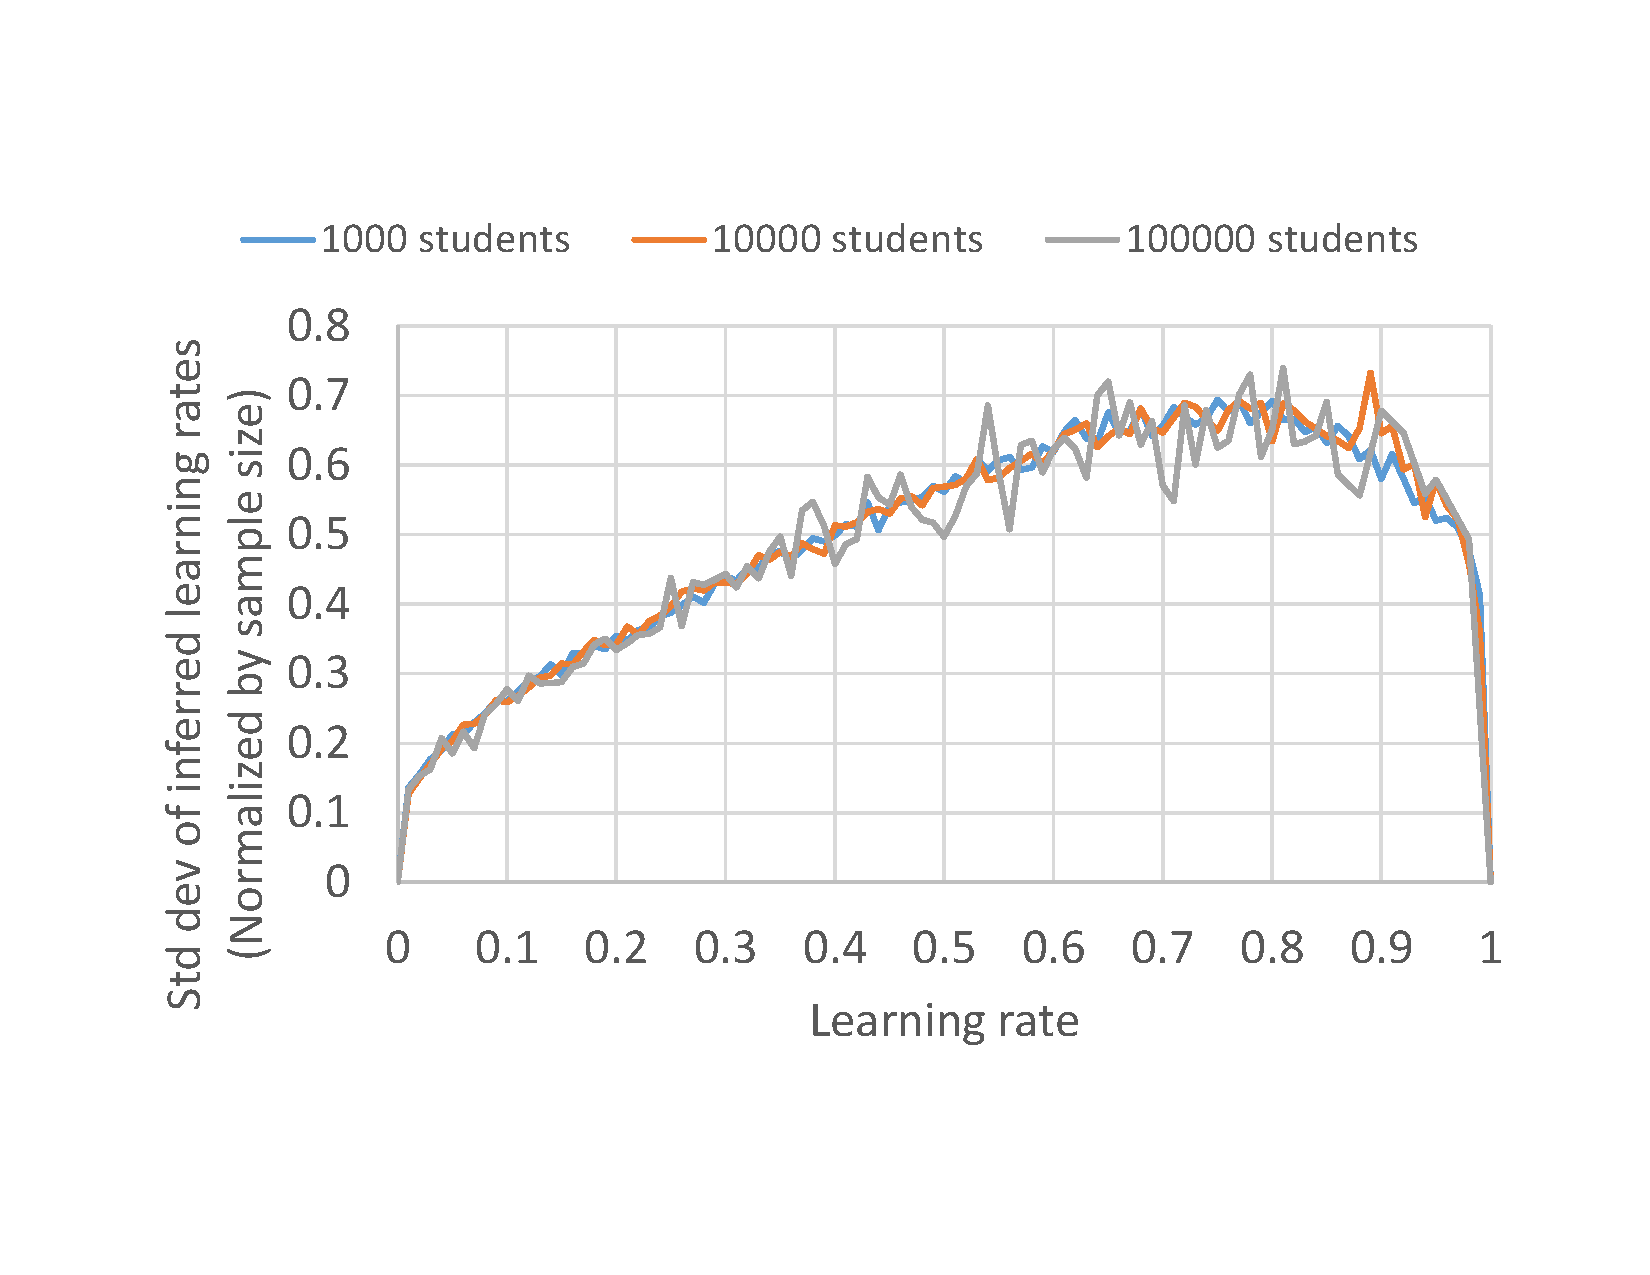
\includegraphics[width=0.5\textwidth]{data/variance4.pdf}
\caption{Here we vary learning rate from 0 to 1, and also vary sample size between the values 1000, 10000, and 100000. The resulting standard deviations are divided by $1/\sqrt{n}$ to normalize for improvement in error due to increased sample size. The resulting curves are nearly identical; the curve for 100000 students appears noisier only because of a lower number of samples (100 instead of 1000). We find no evidence of interaction between sample size and the learning rate.}
\label{fig:variance4}
\end{figure}

\section{Discussion}

Because accuracy is good for parameter values near 0 and 1, this implies that for large enough samples, boundary effects (in which the distribution of error is skewed because values outside of the 0-1 range are not permitted) are not a serious concern.

Interactions between parameters are complex, suggesting that attempting to characterize error in each parameter independently is unlikely to yield good predictions of error. Moreover, attempts to model these interactions analytically may be challenging because they cannot be fit well by low-degree polynomials. A more viable strategy is to form a conservative estimate of error by conducting a grid search of parameter sets that are plausible in a given scenario. On the other hand, once the range of variances at a particular (sufficiently large) sample size is characterized, Figure~\ref{fig:variance3} and Figure~\ref{fig:variance4} show that altering the sample size has a uniform and predictable effect on the error.

The main result that standard deviation is proportional to $1/\sqrt{n}$ suggests that, in order to decrease the margin of error in the estimate of a parameter by a factor of 2, an increase in sample size by a factor of 4 is required. Additionally, Figure~\ref{fig:variance3} shows that achieving even a single valid significant digit in the learning rate requires sample sizes of 1000 students or more. This suggests that studies using BKT with less than 1000 students should be considered carefully for sampling error.

\subsection{Confidence Intervals and Decreasing Training Time}

As noted in Figure~\ref{fig:normal}, provided that the sample size is large enough, the distribution of samples is approximated well by a normal distribution, and the standard deviations computed in synthetic simulations such as the preceding ones can be used to compute confidence intervals containing the true generating parameters (e.g. 95\% of possible values are within two standard deviations). Parameters used in these simulations can be set either by using domain knowledge, and/or by conservatively selecting values that give poor accuracy.

To use our results to decrease training time for a large data set, one approach is to create many small samples (e.g. 100 of size 1000) by sampling uniformly randomly with replacement from the full data set. By training on these, we can estimate the variance of our estimates of each parameter at a sample size of 1000. Then, given a desired level of accuracy and a desired probability of achieving it, we can use $1/\sqrt{n}$ to estimate the best final sample size. If the estimated sample size exceeds the data size, this suggests that more data needs to be gathered.

\section{Conclusions and Future Work}

We've only explored a small part of the space of input parameters that can affect inferred parameter accuracy; the possible interactions between parameters are complex and not fully understood. It would also be useful
to examine different sizes of problem sets, scenarios where different students complete different numbers
of problems, models where parameters such as learning rate and guess/slip are per problem, and models where priors are measured per student (as in Pardos and Heffernan~\cite{conf/um/PardosH10}).

Although it seems intuitive that insufficient sample size can lead to poor parameter estimates with poor predictive power, this deserves verification: it's not clear which errors will damage prediction and which are benign. An empirical synthetic study that examines prediction accuracy could assess this cheaply. Going a step further, it would be useful to simulate an interactive tutoring system and assess a cost function that penalizes the system for both incorrect assessment of mastery, and for failing to assess mastery when it is reached. By applying weights to these error types, the simulation could represent the real-world cost of inaccurate parameters in such a system.

Another important direction is extending our results to real-world data. There are a few approaches. One is to use a very large real-world data set and use its inferred parameters as the ground-truth generating parameters, then examine smaller subsets to determine whether parameters are inferred less accurately. If the BKT model is appropriate, we expect to observe similar relationships between sample size and variance as with our synthetic data. This approach can be compared to one experiment of Ritter~\cite{ritter} (Figure~4), in which they took a large real data set and computed mean-squared error using the best-fit parameters on subsets with smaller number of students ranging from 5 to 500.

There are other approaches to real-world validity. One would be a survey of prior BKT applications, to identify whether there is a consistent relationship between sample size and reported prediction accuracy. A third approach would be a controlled experiment in which two groups of very different sizes each use an ITS, the BKT is trained on the resulting data, and then the groups continue to use the ITS and their learning performance is examined (note however that asymmetric group sizes limit statistical power).

Finally, an analytical model that can explain some of our empirical results---such as the skewed normal distribution of inferred parameter values, the improvements in parameter inference near 0 and 1 parameter values, or the $1/\sqrt{n}$ relationship between sample size and standard deviation---would be a valuable contribution.

\section{Acknowledgments}
We thank Zachary A. Pardos for his \emph{fastHMM} C++ BKT library~\cite{pardosjohnson}, for providing helpful comments on this work, and for designing the assignment which inspired it.

\bibliographystyle{abbrv}
\bibliography{hw2ext}
\end{document}
